\documentclass[10pt]{article}

\usepackage[utf8]{inputenc}
\usepackage{csquotes}
\usepackage[english]{babel}
\usepackage[hidelinks]{hyperref}
\usepackage{graphicx}

\usepackage{amsmath,amssymb}

\usepackage{wrapfig}
\usepackage{algorithm}
\usepackage{algorithmic}

\usepackage[citestyle=numeric]{biblatex}

\title{Simulating Acoustics with Ray-Tracing in Rust}
\author{Kristofer Rye}

\addbibresource{bibliography.bib}

\begin{document}
\maketitle

\begin{abstract}
  \noindent Ray tracing, a common method used in computer graphics to produce
  photo-realistic images, has natural applications to the study of acoustics.
  Sound moving through space can be modeled by particles which represent the
  wavefront as it moves through space, and sufficient numbers of particles can
  produce a well-resolved profile of received sound that is emitted from that
  point.  We implement a primitive simulation system to approximate the
  acoustics of a modeled space and examine its resulting characteristics.
\end{abstract}

\section{Introduction}

Ray tracing is a common method used in the field of computer graphics to
simulate the motion of light through space, and is commonly used to produce
photo-realistic images.  The idea of ray tracing in computer graphics originally
came from the problem of computing the projection of shadows, \cite{Appel1968}
but developed in both accuracy and speed after it was popularized through its
use in computer graphics.  Originally conceived in the field of optics
\cite{Spencer62}, ray tracing eventually reached popularity in cases where it
was practical.  Ray tracing has also seen use in physics research settings,
especially for modeling the propagation of seismic waves, radio signals, and
underwater sound.

A few things about sound make ray tracing particularly useful in the modeling of
acoustics.  First, since sound in air moves at a velocity far less than that of
light, this means its motion through the space can be accurately approximated
with particles moving at non-relativistic speeds.

Rust is a programming language of rising prominence with a stated goal of
``empowering everyone to build reliable and efficient software.'' \cite{Rust}
Rust was selected for this project because of a few key distinguishing factors.
These include Rust's exceptional memory safety guarantees, the inherent
fearlessness of concurrency of Rust code, and the fact that Rust can be compiled
both to native machine code (on x86\_64 and similar devices) as well as
WebAssembly, which allows it to be embedded within the browser rather cleanly.

In addition, Rust's type system, specifically its rich support for generic
functions and generic types, means that all of the algorithms with which we are
concerned can be implemented for all types that support the underlying operation
generics.  For a specific example example, this means that the same
implementation of our intersection algorithm can work in both two and three
dimensions, as it makes use of the dot product which is well-defined in both
dimensions.

\section{Algorithms}

The system we developed allows for the measurement of the acoustics of a modeled
space with a specifiable level of detail.  Wavefronts are approximated as
particles carrying frequency and amplitude data, and are emitted
omni-directionally (uniformly distributed, and randomly) within the space, and
objects are modeled as either spheres (with a given origin and radius) or
collections of triangles.

\begin{wrapfigure}{o}{0.5\textwidth}
  \begin{minipage}{0.5\textwidth}
    \begin{algorithm}[H]
      \caption{The simulation structure}
      \label{simalg}
      \scriptsize
      \begin{algorithmic}
        \STATE Objects $\gets$ [room geometry]
        \STATE Objects $\gets$ [receivers]

        \FOR {emitter $\in$ Emitters}
        \STATE Sounds $\gets$ emitter.emit
        \ENDFOR

        \REPEAT

        \FOR {sound $\in$ Sounds}
        \STATE I $\gets$ []
        \FOR {object $\in$ Objects}
        \STATE I $\gets$ sound.hit?(object)
        \ENDFOR

        \STATE hit $\gets$ I.first

        \IF{hit.object is a Receiver \OR $\text{sound.amplitude} * \text{hit.reflectance} < \epsilon$}
        \STATE hit.object.hits $\gets$ hit
        \STATE Sounds.delete(hit.sound)
        \ELSE
        \STATE hit.sound.bounce(hit.object)
        \ENDIF

        \ENDFOR

        \UNTIL{Sounds $= \varnothing$}
      \end{algorithmic}
    \end{algorithm}
  \end{minipage}
\end{wrapfigure}

Our simulation consists of a loop (Algorithm \ref{simalg}) that continues
endlessly until all sounds emitted at the start of the simulation have either
been received or would be imperceptibly weak by the receiver.  For each
iteration through the simulation loop, every sound ray is checked against every
object in the scene for an intersection (``hit''), and the intersection results
are stored in a container which automatically sorts the stored sounds in
ascending order by time, such as a binary tree.  As a result, the time
complexity of checking every sound with every object has time complexity
$\mathcal{O}(m \cdot n)$ where $m$ denotes the number of sounds and $n$ denotes
the number of objects.  The claim that this worst-case time complexity is the
best possible without advanced techniques needs verification, but hopefully
intuitively makes sense: in short, culling would only remove a certain
proportion of the objects in the scene, but all objects still need to be checked
against all sounds in order to find the earliest hit, since that is what would
happen first.

The algorithms for identifying intersections of sound (approximated by rays) and
surfaces (approximated by triangles and spheres) are taken from relevant
literature sources.  Notably, we use the fast and lightweight algorithm
presented by M\"oller and Trumbore in \cite{raytrialgo}, which can be used not
only to determine \emph{whether} a given ray intersects with a triangle, but
also \emph{exactly where}, and \emph{at exactly what time}, both of which are
relevant to our simulation.  The ray-sphere intersection was derived using
Wolfram Mathematica to generate a parameterized form of the sphere equation with
one parameter (time), and this was then translated into code.  Since a ray can
intersect with a sphere at exactly zero, one, or two points, the intersection
returns both points and the earlier time is selected.  Unit normal vectors are
generated in both intersection algorithms and are used by the scene simulator to
compute in what direction the outgoing ray moves.

One limitation of our system is that it assumes perfectly elastic collisions
with un-movable surroundings, and---perhaps more significantly---that sound
exclusively bounces at a lower amplitude when it interacts with a surrounding.
In reality, a wavefront interacts with the actual materials of the wall on a
highly detailed basis, and the level of detail required proves to be
impractical.  Instead, our system requires that entire surfaces (groups of
triangles) are approximated with a single coefficient representing how much of
the sound they reflect, and as additional detail is needed, additional surfaces
must be added.  Furthermore, we assume exactly one medium with one speed of
sound, which is not wholly realistic.  A given space could have varying speeds
of sound in different areas as factors like lighting induce thermal differences
and air currents.  The difference in sound profile is assumed to be negligible,
but in practice might be somewhat significant.

An alternative or more primitive approach to implementation would have rays
stepping forward an arbitrarily small amount, checking for bounces off each
object at each time step, and moving in accordance with a \emph{computed} speed
of sound, rather than a constant speed of sound.  Such an approach would allow
for the simulator to account for differences in localized temperature and speed
of sound, but since in most time steps no collisions would be observed, a large
amount of time would be wasted checking for those collisions.

\section{Results}

The simulated space is a $20~\mathrm{meter}~\text{long} \times
10~\mathrm{meter}~\text{wide} \times 10~\mathrm{meter}~\text{tall}$ space, with
a front wall, ceiling, and floor each absorbing $20\%$ of the intensity of the
sound that they receive, a back wall absorbing $80\%$ of the sound that hits it,
and left and right walls each absorbing $60\%$ of the sound that hits them.  The
emitter is located $1~\mathrm{m}$ towards the front wall, and the receiver is a
$0.1~\mathrm{m}$-radius sphere, of comparable size to the human head.  According
to the textbook's approximation for reverberation time, the reverberation time
($RT$) of this space would be given by \begin{align*} RT &= 0.161 \frac{V}{A}
  \\ &= 0.161 \frac{2000~\mathrm{m^3}}{(100 + 2 \cdot 200) \cdot .20 + 100 \cdot
    .80 + (2 \cdot 200) \cdot .60~\mathrm{m^2}} \\ &\approx
  .767~\mathrm{s} \end{align*}

When the simulation is run, a configurable number of rays---which, for the sake
of the included figures, is $1,000,000$---is produced by the emitter,
distributed uniformly along a unit sphere and then scaled by the speed of sound.
The simulation is then run to completion, taking approximately $8$ iterations
before all sounds have been absorbed, which represents approximately $8$ bounces
off of walls before the sound is received.  The simulation subroutine then
yields back a table containing the observed ``hit'' data (including what
intensity was recorded) and time of the observation.  These data can then be
plotted using a tool like gnuplot with time on the horizontal axis and intensity
on a logarithmic scale on the vertical axis, producing the following figures.

\begin{wrapfigure}{o}{0.5\textwidth}
  \begin{center}
    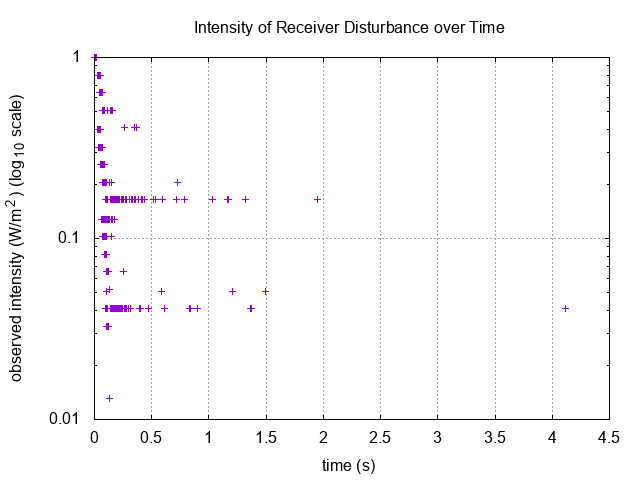
\includegraphics[width=0.48\textwidth]{results-paper}
  \end{center}
  \caption{Simulation results}
  \label{unconstrained}
\end{wrapfigure}

The first figure, Figure \ref{unconstrained}, shows one run of the simulation.
Nearly all of the sound is received within the first two seconds, but the
logarithmic scale demonstrates how since nearly all of the sound is reflected
around only a few times, only three orders of magnitude on intensity are lost,
representing a loss of only $30~\mathrm{dB}$ of loudness.  Likewise, the
intensity levels observed are quantized onto a handful of levels that can be
seen as horizontal groupings.  Since the geometry of the space is incredibly
simple, each intensity level corresponds to a certain, countable and finite
number of bounces off of a surface, and there is not much variability as there
are only six surfaces with which a sound wave can interact with.
\begin{wrapfigure}{i}{0.5\textwidth}
  \begin{center}
    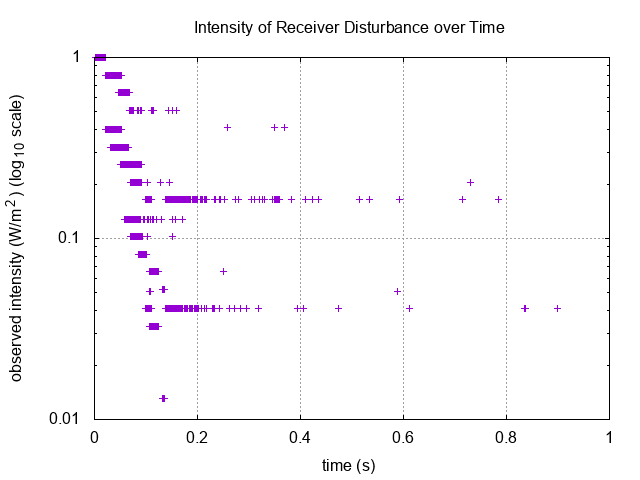
\includegraphics[width=0.48\textwidth]{results-paper-constrained}
  \end{center}
  \caption{Simulation results, constrained to $[0, 2)$ seconds}
  \label{constrained}
\end{wrapfigure}

Figure $\ref{constrained}$ displays the same results, constrained to only the
first two seconds on the horizontal axis.  Here various groupings of sound waves
can be observed, the first of highest intensity from a time near zero seconds to
a time near $0.1$ seconds, and with the second highest intensities coming
shortly after that.  There is also a significant group of particles which
reached the receiver with an intensity between $0.1$ and $0.2~\mathrm{W/m^2}$,
corresponding to a bounce off the ceiling and the floor, or the front wall and
either the floor or the ceiling.  An additional long group of particles which
reached the receiver with roughly $0.03~\mathrm{W/m^2}$ corresponding to a
bounce off the back wall, with varying angles of incidence corresponding to a
longer time delay.  Adjusting the reflectance parameters of the ceiling and
floor produces other groupings like these at different intensity levels,
confirming how they are formed.  Indeed, most of the sound is observed to
dissipate by $0.767$ seconds, in accordance with the prediction by the textbook.

\subsection{Limitations}

Our system does not support filtering different frequencies at different levels,
however it would be trivial to extend it to work as such.  When computing the
resulting amplitude, instead of simply multiplying by a constant, a more
complicated calculation could be performed based on linear interpolation over
known reflectances at known frequencies, for example.  We also assume the same
amount is absorbed by a surface with a blow by a wave compared to a head-on
wavefront, which is not necessarily the case in optical ray tracing.
Furthermore, as mentioned before, our simulation only runs once with one
wavefront, simulating the sound of a sharp change in pressure, such as a
piercing explosion, at $120~\mathrm{dB}$.  This does not model most musical
sounds, which would consist of a fundamental and its partial series based on the
timbre of the instrument.  Further modeling would be required to describe how
the timbre of transmitted sound changes as it goes through the space.

\section{Conclusion}

We have implemented a ray-tracing acoustics engine that produces somewhat
realistic results in a simple but still complete example.  Our system allows for
maximum configurability and uses relatively fast technologies so that its level
of detail can still remain high as more complex simulations are performed.
Indeed, ray tracing proves very promising for validating assumptions about
spatial acoustics in the design phase rather than in the implementation phase of
construction, which means that ray tracing has a lot of potential uses in the
study of acoustics as it relates to architectural design.

\printbibliography

\end{document}
